\documentclass{article}


%\usepackage{arxiv}

\usepackage[utf8]{inputenc} % allow utf-8 input
\usepackage[T1]{fontenc}    % use 8-bit T1 fonts
\usepackage{hyperref}       % hyperlinks
\usepackage{url}            % simple URL typesetting
\usepackage{booktabs}       % professional-quality tables
\usepackage{amsfonts}       % blackboard math symbols
\usepackage{nicefrac}       % compact symbols for 1/2, etc.
\usepackage{microtype}      % microtypography
\usepackage{lipsum}
\usepackage{algorithm}
\usepackage[english]{babel}
\usepackage[noend]{algpseudocode}
\usepackage[toc,page]{appendix}
\usepackage{graphicx,epstopdf,caption}
\usepackage{float,colortbl}
\usepackage{hyperref}
\usepackage{amssymb}
\usepackage{amsmath}
\usepackage{amsthm}
\usepackage{bbm}
\usepackage{fullpage}
\usepackage{enumitem}
\usepackage{caption}
\usepackage{subcaption}
\usepackage{multirow}
\usepackage{makecell}
\usepackage{courier}

\usepackage{setspace}
\doublespacing

\usepackage{titling}
\setlength{\droptitle}{-5em}   % This is your set screw
\usepackage[left=1in, right=1in, top=1in, bottom=1in]{geometry}


\usepackage[natbib=true,style=authoryear, useprefix=true, maxcitenames=2, backend=biber]{biblatex}
\addbibresource{references.bib}

\title{Textual Causal Inference about Readers' Interest on News Articles}


\author{
	Yu Yang\thanks{School of Statistics, University of Minnesota, \href{mailto:yang6367@umn.edu}{yang6367@umn.edu}}
}
\date{}

\begin{document}
	\maketitle
	\vspace{-5em}
	%\begin{abstract}
	%For this, ...
	%\end{abstract}
	%
	%
	%% keywords can be removed
	%\keywords{Textual Causal Inference \and CNN/Daily Mail}
	
	\section{Introduction}
	
	A major challenge in causal inference is to deal with the biases caused by confounders. A golden method to eliminate the confounding bias is to perform randomized controlled trials, which can often be infeasible or unethical. In face of this, researchers turn to observational data and try to make adjustment for the confounders. Popular methods include regression adjustment, propensity score regression adjustment, inverse propensity score weighting, and matching. 
	
	In recent years, researchers have been trying to dig information out of textual data, which they believe can serve as a surrogate for the latent confounders. For example, \cite{olteanu2017distilling} investigated how people's current word uses would affect their future word uses, where they measured the confounder - past word uses - from Twitter posts. And \cite{veitch2020adapting} used articles' content to measure the subjects so as to infer how the presence of a theorem affects the rate of acceptance. However, despite of these progress, several challenges remain. (1) Text data by nature is of high dimension and requires a conversion into a meaningful lower-dimensional representation vector. (2) It remains an open question how to evaluate different causal inference methods under the textual scenario \parencite{keith2020text} and there is no solid best-performing inference method from a theoretical perspective. 
	
	This paper focuses on how the length of an article affects readers' interest to read it, which is of critical values to publishers, especially news article publishers, in terms of getting more readers and higher click rate for their articles. In particular, we use the CNN/Daily Mail news articles dataset \parencite{nallapati2016abstractive} for this study, and we consider the treatment as whether the article is longer than 800 tokens\footnote{A token is a sequence of characters in the document that are grouped together as a semantic unit. We may obtain the tokens of a sentence by chopping it up into pieces and throwing away special characters such as punctuation and whitespace. For example, we may process the sentence "I like winter and snow." into 5 tokens: ["I", "like", "winter", "and", "snow"].} and the outcome as whether the readers will read it. One confounder could be the topics of the paper - for example, sports news articles tend to be shorter and at the same time may have a large number of fans choosing to read them. Since there is no solid conclusion on which adjustment strategy works the best under the textual scenario, we perform a series of simulations\footnote{Check the code in Github: \url{https://github.umn.edu/YANG6367/PUBH8485/tree/master/project}.} to investigate the most appropriate method for this particular problem.
	
	The rest of the paper goes as follows. Section \ref{section: methods} introduces the simulation mechanism and the modeling methods in details; Section \ref{section: results} demonstrates the performance of different adjustment methods by simulation metrics; Section \ref{section: conclusion} concludes the paper with some discussion.
	
	\section{Simulation Mechanism and Methods}\label{section: methods}
	In this section, we describe the simulation mechanism and the estimation methods in the methodology level and will go into technical details in Section \ref{section: results}. 
	\subsection{Simulation Mechanism}
	Since we don't know the ground-truth causal effects, it would be difficult to compare different effect estimation methods empirically. Therefore, similar to \cite{veitch2020adapting}, we approach this problem with semi-synthetic data: we use the real news articles but simulate the outcome based on the treatment and the confounders, and then we use the simulated data to estimate ATE.
	
	We use the CNN/Daily Mail dataset \parencite{nallapati2016abstractive} for simulation, which consists of 312,085 online news articles. As in \cite{see2017get}, we use the non-anonymized version of the data, which is split into 287,225, 13,368, and 11,490 examples for training, validation and testing respectively.  For each news article, we can obtain two attributes:
	\begin{enumerate}
		\item length: the total number of tokens in the article.
		\item hot topic inclusion: whether the article contains "government", "crime", "economic", "game", "health".
	\end{enumerate}
	
	Let $t_i$ denote whether or not the $i$th article has more than 800 tokens and let binary vectors $z_i$ denote the inclusion of "politics", "crime", "economics", "game" and "health", with $z_{ik}=1$ indicating the inclusion of the $k$th topic type in the $i$th article. Note that 800 is chosen to be close to the median of the document length in the training set in order to keep the treatment balanced.
	
	First, for each stratum of $z$ (in total 32 strata), we calculate the true propensity score $\pi(z)$, which equals to the proportion of cases with $t_i = 1$ in the training set. Then, we simulate $Y_i$ following the model: 
	\begin{equation}\label{eq: simulation}
		Y_i \sim Bernoulli (\sigma (\alpha t_i + \beta \pi(z_i) + \gamma)),
	\end{equation}
	where $\sigma(\cdot)$ is the sigmoid function. The parameter $\alpha$ controls the treatment effect. The parameter $\beta$ is used to control the level of confounding, implying the bias had we not adjust for the confounding. And the parameters $\gamma$ is to control the outcome probabilities to stay close to the real-life scenario.
	
	\subsection{Estimation Methods}
	\textbf{Topic Model} To start with, we train a topic model to learn the topic embedding vector for each article, which is then used as the surrogate for the confounders. There are many different topic embedding methods, such pLSA \parencite{hofmann1999probabilistic}, LDA \parencite{blei2003latent}, Replicated Softmax \parencite{hinton2009replicated}, neural-based topic models \parencite{miao2017discovering} and ETM \parencite{dieng2020topic}. We consider the ETM model, which builds on top of the recent progress in pre-trained word embedding areas and has been shown to have good topic interpretation as well as robustness to stop words\footnote{Stop words usually carry little useful semantic information but will affect the quality of topic models if not taken care of. Examples include: "a", "the", "is", "are" and etc.} \parencite{dieng2020topic}. In more detail, this model assumes the generation story of the $d$th document to be the following ($d = 1, \cdots, D$):
	\begin{enumerate}
		\item Draw the topic proportion vector $\theta_d \sim LN(0, I_K)$, namely, $\delta_d \sim N(0, I_K), \theta_d = \text{softmax} (\delta_d)$.
		\item For the $n$th word $w_{dn}$ in the document: 
		\begin{enumerate}
			\item Draw the topic assignment from a multinomial distribution characterized by $\theta_d$: $\xi_{dn} \sim \text{Multinomial}(\theta_d)$.
			\item Draw the word from a multinomial distribution: $w_{dn} \sim \text{Multinomial}(\text{softmax} (\rho^T \alpha_{\xi_{dn}}))$.
		\end{enumerate}
	\end{enumerate}
	where $D$ is the total number of documents in the data set, $K \in \mathbb{R}$ is the number of topics, $\rho \in \mathbb{R}^{L\times V}$ is the word embedding matrix, with $L$ being the word embedding size and $V$ being the vocabulary size, and $\alpha_i \in \mathbb{R}^L$ is the  embedding vector of the $i$th topic, $i = 1, \cdots, K$.
	
	We use variational inference \parencite{jordan1999introduction, wainwright2008graphical} to fit ETM, where we posit the family of the topic proportion distribution $q(\delta_d; \textbf{w}_d, \nu)$ to be Gaussian and then use amortized variational inference \parencite{kingma2013auto, rezende2014stochastic} to estimate the parameters (see Section 5 in \cite{dieng2020topic} for details). The inference network takes the normalized bag-of-word representation\footnote{For each word in the vocabulary, count how many times it appears in the document.} of the document as the input and outputs the mean and variance of $\delta_d$, which can then be used to generate the topic proportion vector $\theta_d$ through sampling and transformation.
	
	\textbf{Adjustment Methods} After getting the topic proportion vectors, we then build a neural classifier as the propensity score model, with the topic proportion vector being the input\footnote{I have also tried using the weighted topic vector $\sum_i^K \theta_{di} \alpha_i \in \mathbb{R}^L$ as the representation vector, but the result is not as good. Check \url{https://github.umn.edu/YANG6367/PUBH8485/tree/master/project/etm-ps} for more details.} and whether the length of the article exceeds 800 tokens being the output. Finally, with the propensity score model at hand, we compare the performance of four average treatment effect (ATE) estimation methods: (1) Propensity Score Regression Adjustment (PSReg); (2) Propensity Score Stratification (PSS); (3) Inverse Probability Weighting (IPW); (4) Inverse Probability Weighting variant (IPW2).
	
	
	\section{Experiments and Results}\label{section: results}
	In this section, we describe the technical details of the experiments and the results. 
	
	\subsection{Simulation Setup}
		
	We consider two schemes to set parameters in Equation \ref{eq: simulation}. For both schemes, we fix $\alpha = -1$ and vary $\beta$ from 1 to 10 to investigate how different methods perform under different confounding levels. Regarding $\gamma$, for the first scheme, we vary it along with $\beta$ to keep $\overline{Y}$  nearly constant at 0.265, while for the second scheme, we vary it along with $\beta$ to keep the ground-truth ATE (defined later) nearly constant at -0.2. Therefore, we would consider 20 settings in total. And for each setting, we simulate the data with 100 repetitions and report the mean and standard error of the ATE estimation results. 
	
	\subsection{Model Details}
	\textbf{ETM} We use the pre-trained RoBERTa model \parencite{liu2019roberta} to initialize the word embedding matrix $\rho$ and the tokenizer\footnote{A tokenizer performs tokenization and transforms a document into a list of tokens. In the paper, we use the one implemented by Hugging Face: \url{https://huggingface.co/docs/transformers/model_doc/roberta}.}. The vocabulary size $V$ is 50265 and the word embedding size is 768, and therefore, $\rho\in \mathbb{R}^{50265 \times 768}$. The total number of topics $K$ is set as 300. To perform amortized variational inference, we build a three-layer neural network to model the mean and variance of $\theta_d$ and use the reparameterization trick \parencite{kingma2013auto, titsias2014doubly} and stochastic optimization to update the parameters. Let \texttt{FC k-l} denotes a $k\times l$ fully connected layer. The network consists of \texttt{FC 50265-800, ReLU, FC 800-800, ReLU, FC 800-300}. The model is trained on the training set for 10 epochs and parameters are tuned using the validation set. The learning rate is initialized as 0.005 and decreases exponentially with rate 0.999. After training, each article in the training set is passed to the trained model to obtain its corresponding topic proportion vector $\theta_d$. 
	
	\textbf{Propensity Score Model} The neural propensity score model is a three-layer network consisting of \texttt{FC 300-1000, BatchNorm\footnote{One technique to make the network training faster and more stable.}, LeakyReLU, FC 1000-300, BatchNorm, LeakyReLU, FC 300-1, Sigmoid}. This model takes the topic proportion vector as the input and outputs the probability that the document is longer than 800 tokens. The training loss function is the Binary Cross Entropy \footnote{As defined in PyTorch Documentation \url{https://pytorch.org/docs/stable/generated/torch.nn.BCELoss.html}} between the target and the estimated probabilities. This model is trained on the training set for 5 epochs and the initial learning rate is 0.02, which then decreases exponentially with rate 0.999. After training, we apply the trained model to the topic proportion vectors and get the corresponding propensity scores. 
	
	\textbf{ATE Estimation} For the PSReg method, we consider the interaction between the treatment and the restricted cubic spline (of order 5) transformation of the estimated propensity score in the logistic regression model. For the PSS method, we divide the data into deciles based on the estimated propensity scores. For the IPW method, $\mathbb{E}[Y^1]$ is estimated by $\frac{1}{D} \sum_{d=1}^D\frac{t_i Y_i}{\hat{\pi_i}}$, while for the IPW2 method, $\mathbb{E}[Y^1]$ is estimated by $\frac{1}{D}\sum_{d=1}^D \frac{t_i Y_i}{\hat{\pi_i}} / (\frac{1}{D}  \sum_{d=1}^D\frac{t_i}{\hat{\pi_i}})$.
	
	\subsection{Results}
	For each of the simulation setting, we compute the ground-truth average treatment effect as $\frac{1}{D} \sum_{d=1}^D [\sigma(\alpha t_i + \beta \pi(z_i) + \gamma) - \sigma(\beta \pi(z_i) + \gamma)]$ and apply the four ATE estimation methods to the simulated data with the trained propensity score model. The results for Scheme 1 are shown in Table \ref{tab:results} and Figure \ref{fig:results} and the results for Scheme 2 are shown in Table \ref{tab:results2} and Figure \ref{fig:results2} in the Appendix. We can see that 
	
	\begin{enumerate}
		\item all methods help reduce the confounding bias, and among them, IPW works the best in general under both schemes; 
		\item the performance of PSReg, PSS, and IPW2 are very similar for all $\beta$ values under both schemes;
		\item if we hold the ground-truth ATE almost constant, then as shown in Figure \ref{fig:results2}, when $\beta$ increases, the confounding bias, suggested by the difference between the truth and the unadjusted method, increases, which matches how we simulate the data;
		\item still from Figure  \ref{fig:results2}, as $\beta$ increases, the absolute value of the estimated ATEs given by all four methods become smaller. This implies that large confounding biases tend to eliminate the treatment effect in this case.
	\end{enumerate}
	

	
	\section{Discussion}\label{section: conclusion}
	In this paper, we adapt a modern topic model to measure the confounding effect and investigate how articles' lengths affect readers' interest. We have run a simulation study to examine the performance of different confounding adjustment methods and we find that IPW seems to work the best among its cohorts. 
	
	There are several future work directions. First, we may try some other topic models  and check how the choice of topic models affects the treatment effect estimation. Second, we only consider adjustment methods based on propensity scores in this paper and we may include more, such as regression adjustment and matching. Finally, we focus on the CNN/Daily Mail Dataset in this paper and it is worthwhile to investigate whether our findings apply to the other data sets as well. 
	
	\newpage   % to set a new page
	
	
	\printbibliography
	
	\newpage
	\section{Appendix}
	
	\begin{table}[H]
		\centering
		\begin{tabular}{ccccp{15mm}||cp{15mm}p{15mm}p{15mm}p{15mm}p{15mm}}
			\hline
			& $\alpha$ & $\beta$ & $\gamma$ & $\overline{Y}$ & Truth & Unadjusted & PSReg & PSS & IPW & IPW2 \\ \hline 
			\textsl{Setting 1} & -1 & 1 & -1 & 0.2793\newline (0.00084) & -0.1971 & -0.1873\newline (0.00176) & -0.1886\newline (0.00191) & -0.1886\newline (0.00192) & -0.2107\newline (0.00196) & \textbf{-0.1887}\newline (0.00193) \\ 
			\textsl{Setting 2} & -1 & 2 & -1.6 & 0.2658\newline (0.00086) & -0.19 & -0.1704\newline (0.00167) & -0.1731\newline (0.00183) & -0.1731\newline (0.00183) & \textbf{-0.1941}\newline (0.00188) & -0.1732\newline (0.00185) \\ 
			\textsl{Setting 3} & -1 & 3 & -2.1 & 0.2721\newline (8e-04) & -0.1907 & -0.1606\newline (0.00169) & -0.1648\newline (0.00179) & -0.1648\newline (0.00181) & \textbf{-0.1862}\newline (0.00182) & -0.165\newline (0.0018) \\ 
			\textsl{Setting 4} & -1 & 4 & -2.7 & 0.2606\newline (0.00075) & -0.1826 & -0.1432\newline (0.00168) & -0.1488\newline (0.00179) & -0.1488\newline (0.0018) &\textbf{ -0.1693}\newline (0.00182) & -0.149\newline (0.00179) \\ 
			\textsl{Setting 5} & -1 & 5 & -3.2 & 0.2684\newline (0.00077) & -0.1818 & -0.1321\newline (0.00178) & -0.1394\newline (0.00188) & -0.1393\newline (0.00189) & \textbf{-0.1604}\newline (0.00191) & -0.1397\newline (0.00189) \\ 
			\textsl{Setting 6} & -1 & 6 & -3.75 & 0.2677\newline (0.00073) & -0.1766 & -0.1175\newline (0.00175) & -0.1264\newline (0.00183) & -0.1262\newline (0.00184) & \textbf{-0.1472}\newline (0.00186) & -0.1266\newline (0.00183) \\ 
			\textsl{Setting 7} & -1 & 7 & -4.3 & 0.2675\newline (0.00079) & -0.171 & -0.103\newline (0.00174) & -0.1133\newline (0.00179) & -0.1131\newline (0.0018) & \textbf{-0.1341}\newline (0.00182) & -0.1136\newline (0.0018) \\ 
			\textsl{Setting 8} & -1 & 8 & -4.85 & 0.2678\newline (0.00073) & -0.1652 & -0.0887\newline (0.00164) & -0.1005\newline (0.00174) & -0.1003\newline (0.00174) & \textbf{-0.1212}\newline (0.00177) & -0.1009\newline (0.00175) \\ 
			\textsl{Setting 9} & -1 & 9 & -5.4 & 0.2686\newline (0.00068) & -0.1592 & -0.0748\newline (0.00161) & -0.0881\newline (0.00184) & -0.0878\newline (0.0018) & \textbf{-0.1088}\newline (0.00188) & -0.0885\newline (0.00186) \\ 
			\textsl{Setting 10} & -1 & 10 & -6 & 0.2619\newline (7e-04) & -0.1508 & -0.0599\newline (0.00149) & -0.0745\newline (0.00174) & -0.0741\newline (0.0017) & \textbf{-0.0946}\newline (0.00179) & -0.0749\newline (0.00177) \\ \hline
			
		\end{tabular}
		\vspace{1em}
		\caption{\textbf{Scheme 1}(holding $\overline{Y}$ nearly constant at 0.265) Comparison results of ATE estimation methods. The bold numbers represent the one that is the closet to the ground-truth ATE and the numbers in the parentheses are the standard errors from 100 repetitions (with different seeds). }
		\label{tab:results}
	\end{table}
	
		
	
	\begin{figure}[H]
		\centering
		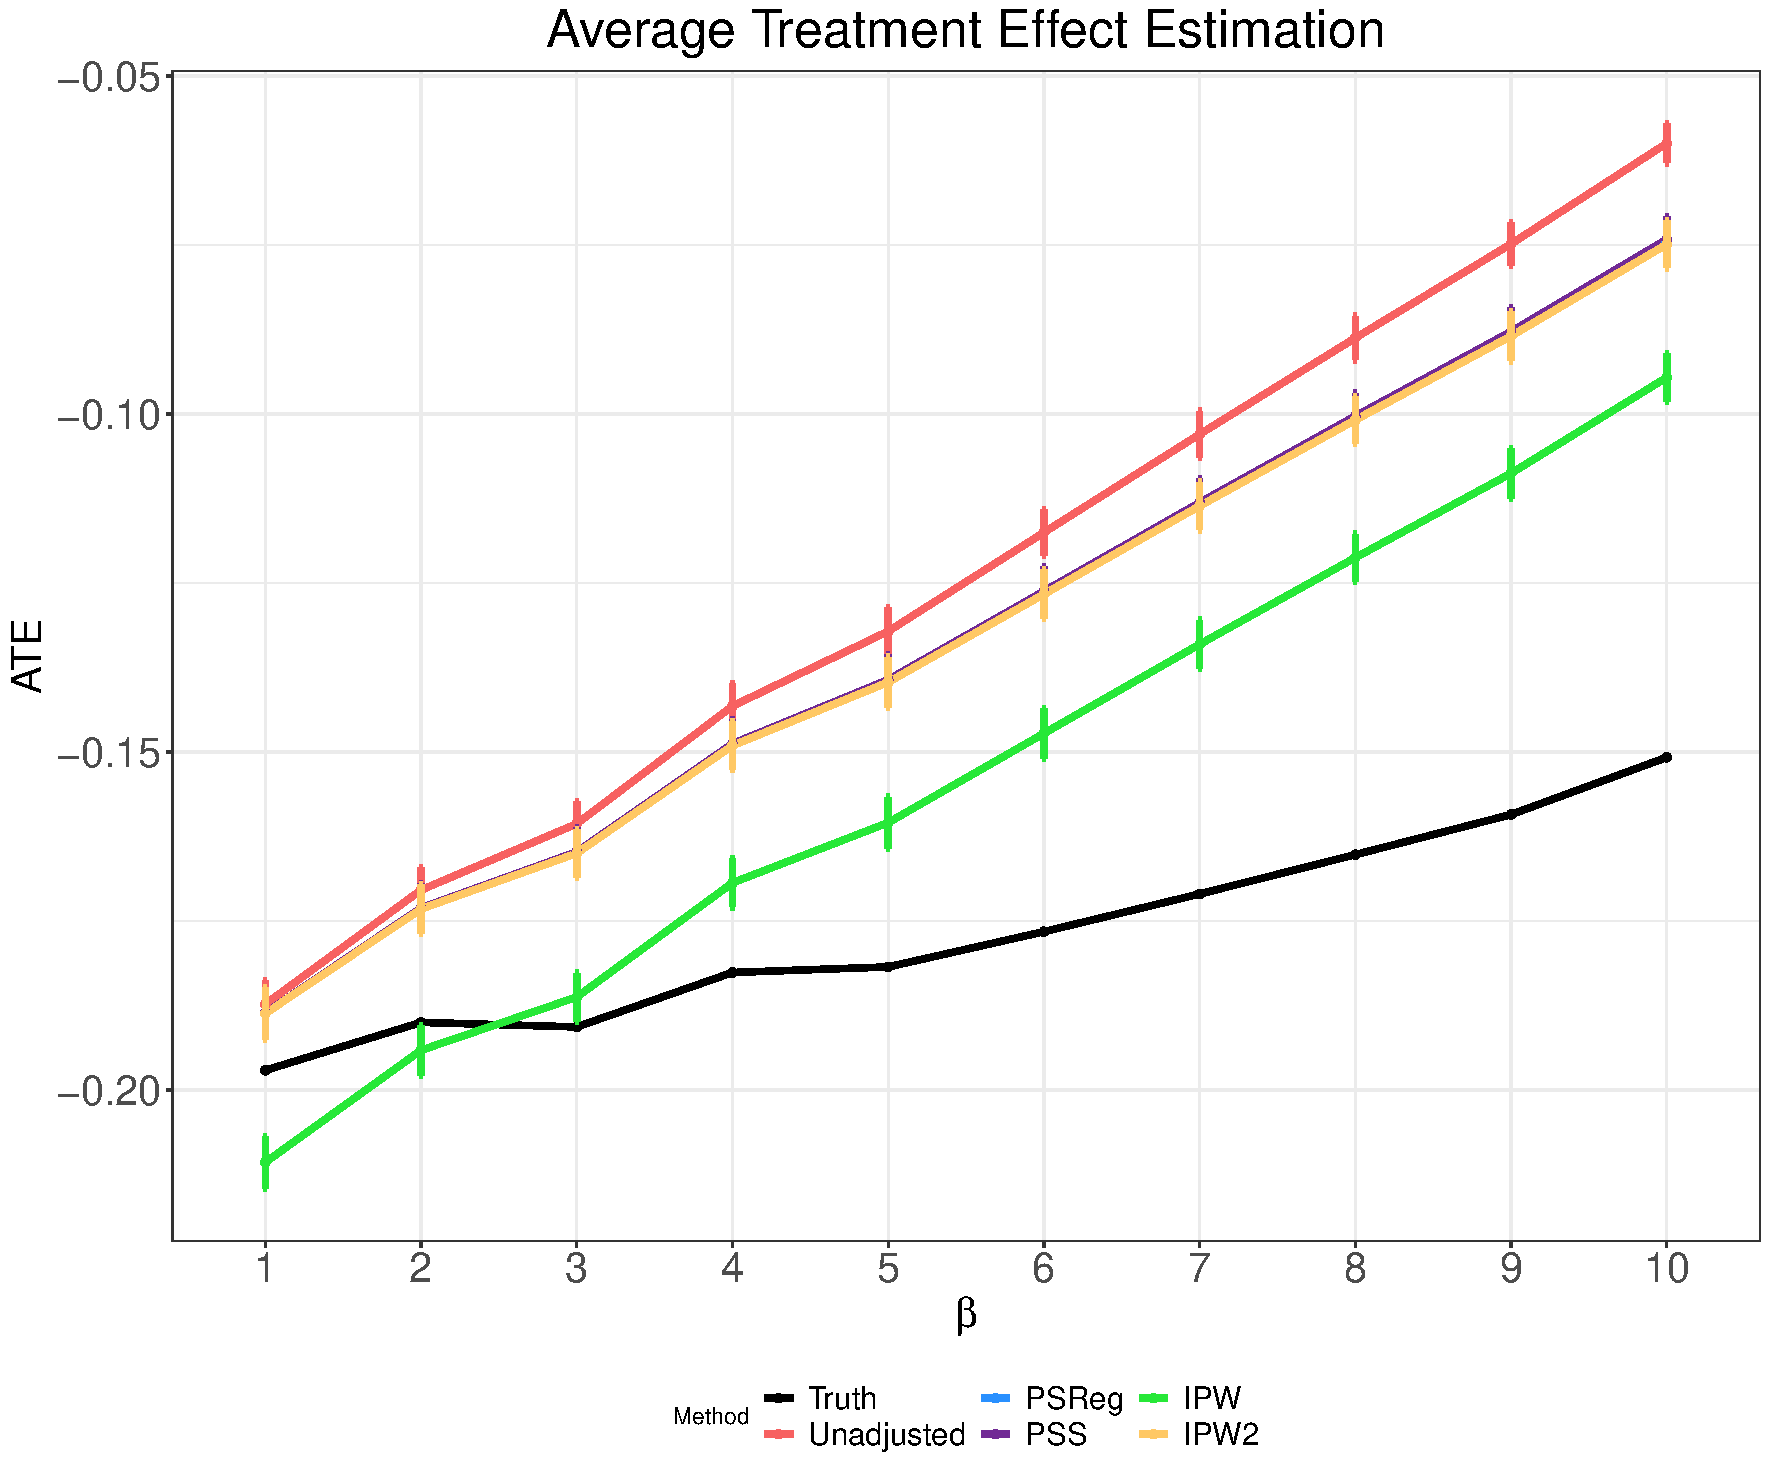
\includegraphics[scale=0.5]{../results/ate_results.pdf}
		\caption{\textbf{Scheme 1} (holding $\overline{Y}$ nearly constant at 0.265) ATE Estimation Comparison. The vertical bars are the 95\% confidence intervals. }
		\label{fig:results}
	\end{figure}

	
	\begin{table}[H]
		\centering
		\begin{tabular}{ccccp{15mm}||cp{15mm}p{15mm}p{15mm}p{15mm}p{15mm}}
			\hline
			& $\alpha$ & $\beta$ & $\gamma$ & $\overline{Y}$ & Truth & Unadjusted & PSReg & PSS & IPW & IPW2 \\ \hline 
			\textsl{Setting 1} & -1 & 1 & -1 & 0.2793 \newline (0.00084) & -0.1971 & -0.1873 \newline (0.00176) & -0.1886 \newline (0.00191) & -0.1886 \newline (0.00192) & -0.2107 \newline (0.00196) & \textbf{-0.1887} \newline (0.00193) \\ 
			\textsl{Setting 2} & -1 & 2 & -1.5 & 0.2848 \newline (0.00083) & -0.1983 & -0.178 \newline (0.00175) & -0.1808 \newline (0.00186) & -0.1808 \newline (0.00187) & \textbf{-0.2033} \newline (0.0019) & -0.1809 \newline (0.00187) \\ 
			\textsl{Setting 3} & -1 & 3 & -2 & 0.2912 \newline (8e-04) & -0.1985 & -0.1677 \newline (0.00164) & -0.1721 \newline (0.00175) & -0.172 \newline (0.00176) & \textbf{-0.1949} \newline (0.00178) & -0.1722 \newline (0.00176) \\ 
			\textsl{Setting 4} & -1 & 4 & -2.47 & 0.3042 \newline (0.00085) & -0.1998 & -0.1579 \newline (0.00175) & -0.1639 \newline (0.00192) & -0.1638 \newline (0.00192) &\textbf{ -0.1877} \newline (0.00194) & -0.1641 \newline (0.00192) \\ 
			\textsl{Setting 5} & -1 & 5 & -2.95 & 0.3158 \newline (0.00082) & -0.199 & -0.1463 \newline (0.00174) & -0.154 \newline (0.00198) & -0.1539 \newline (0.00197) & \textbf{-0.1786} \newline (0.00202) & -0.1542 \newline (0.002) \\ 
			\textsl{Setting 6} & -1 & 6 & -3.4 & 0.3334 \newline (0.00085) & -0.1986 & -0.1352 \newline (0.00177) & -0.1446 \newline (0.002) & -0.1444 \newline (0.00198) &\textbf{ -0.1704} \newline (0.00203) & -0.1449 \newline (0.00201) \\ 
			\textsl{Setting 7} & -1 & 7 & -3.8 & 0.361 \newline (0.00084) & -0.1992 & -0.1254 \newline (0.00183) & -0.1364 \newline (0.00203) & -0.1362 \newline (0.002) & \textbf{-0.1642} \newline (0.00205) & -0.1368 \newline (0.00204) \\ 
			\textsl{Setting 8} & -1 & 8 & -4.15 & 0.3979 \newline (0.00079) & -0.1997 & -0.1164 \newline (0.00176) & -0.1289 \newline (0.00196) & -0.1286 \newline (0.00193) & \textbf{-0.1592} \newline (0.00196) & -0.1292 \newline (0.00195) \\ 
			\textsl{Setting 9} & -1 & 9 & -4.45 & 0.4436 \newline (8e-04) & -0.1991 & -0.1083 \newline (0.00183) & -0.1217 \newline (0.00203) & -0.1214 \newline (0.00198) & \textbf{-0.1553} \newline (0.00201) & -0.122 \newline (0.002) \\ 
			\textsl{Setting 10} & -1 & 10 & -4.5 & 0.5372 \newline (0.00083) & -0.1978 & -0.1055 \newline (0.00188) & -0.1182 \newline (0.00204) & -0.118 \newline (0.002) & \textbf{-0.1586} \newline (0.00206) & -0.1186 \newline (0.00205) \\  \hline
		\end{tabular}
		\vspace{1em}
		\caption{\textbf{Scheme 2} (holding ground-truth ATE nearly constant at -0.2)  Comparison results of ATE estimation methods. The bold numbers represent the one that is the closet to the ground-truth ATE and the numbers in the parentheses are the standard errors from 100 repetitions (with different seeds). }
		\label{tab:results2}
	\end{table}
	
		
	\begin{figure}[H]
		\centering
		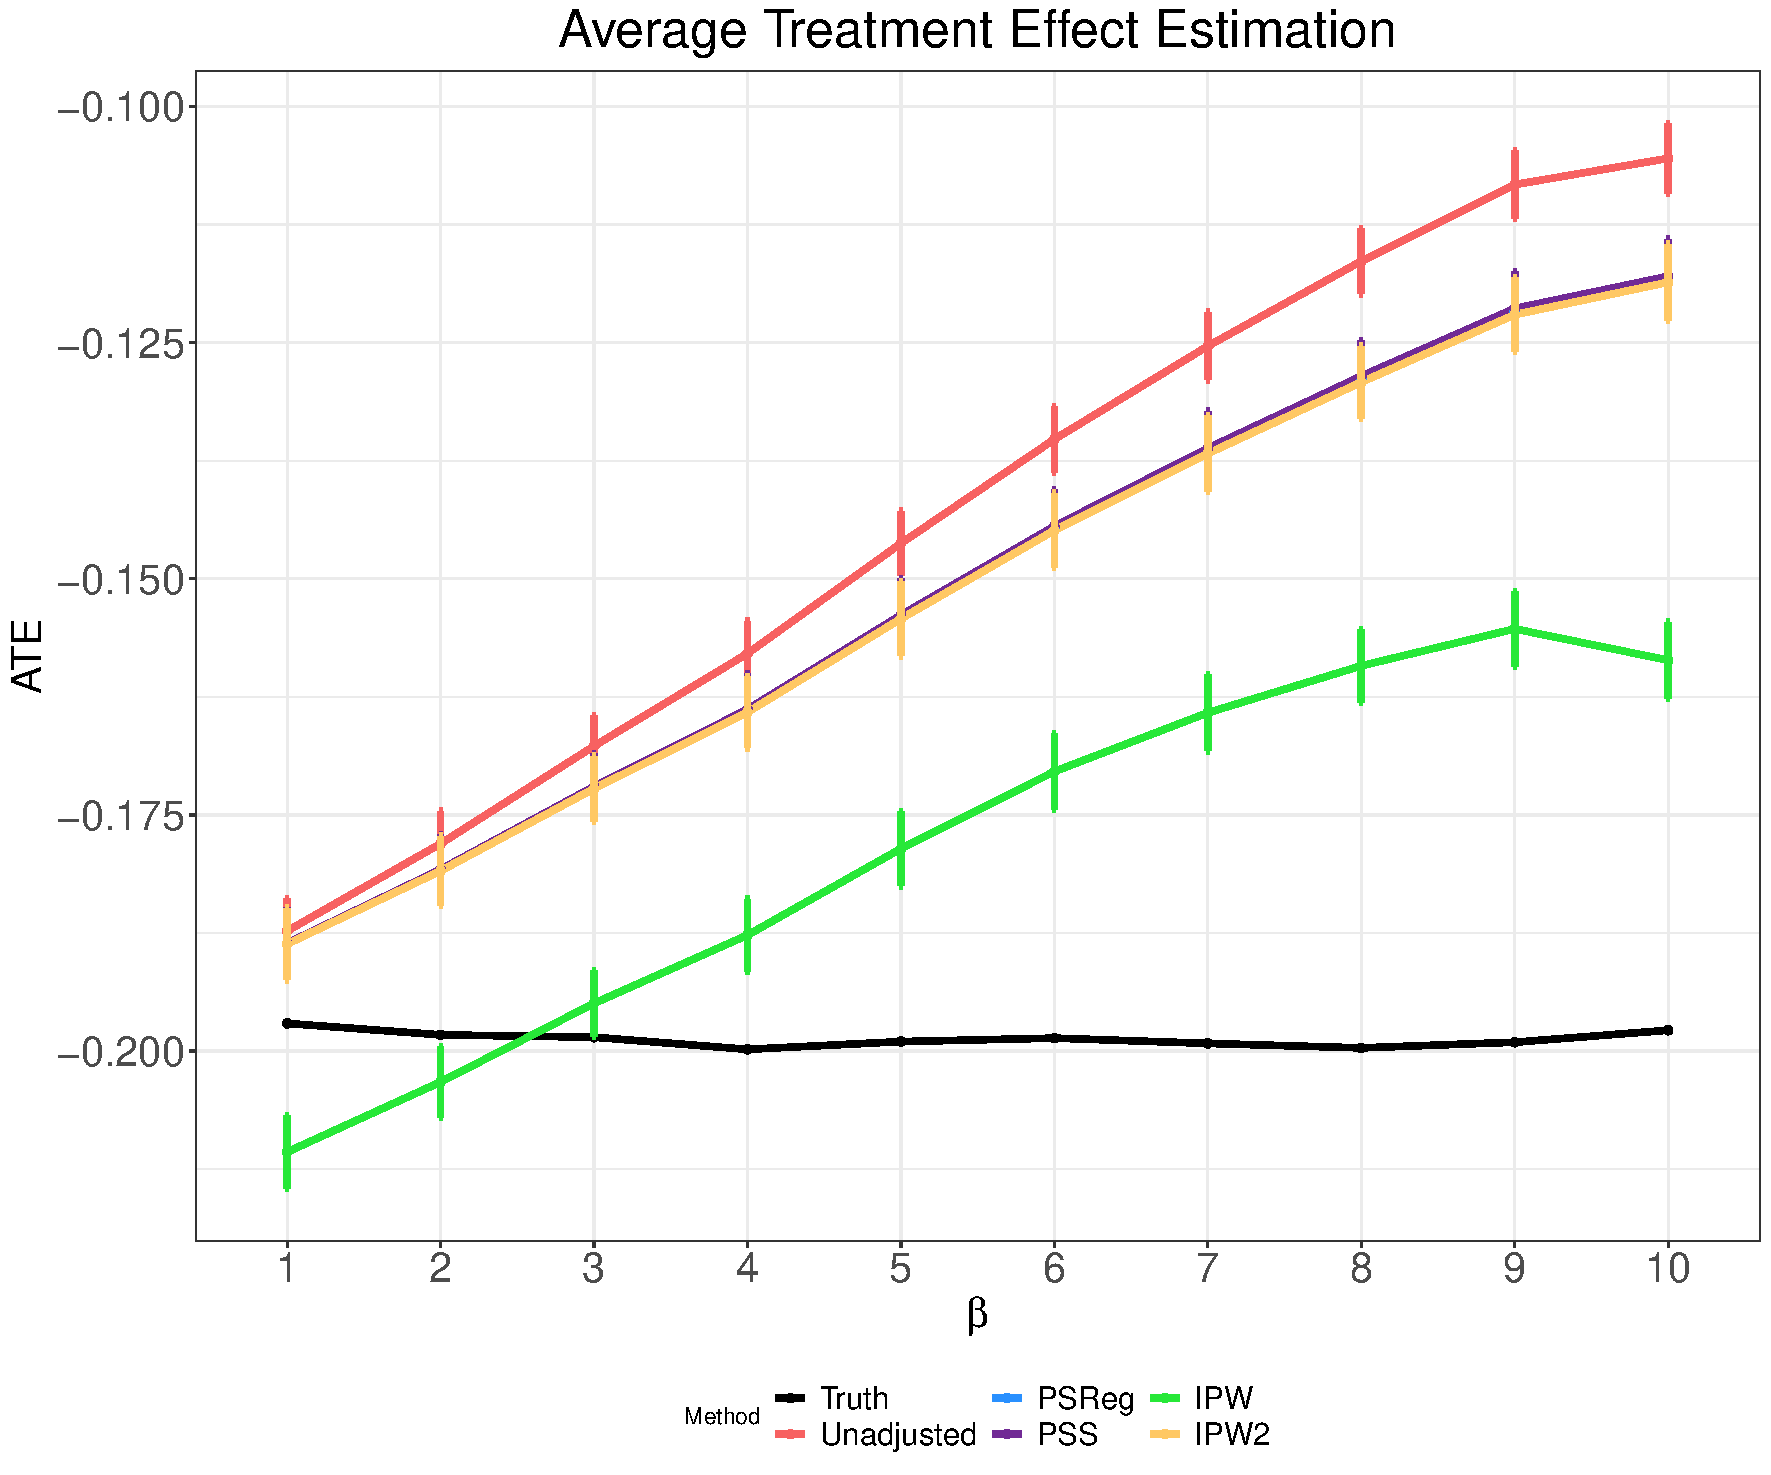
\includegraphics[scale=0.5]{../results/ate_results2.pdf}
		\caption{\textbf{Scheme 2} (holding ground-truth ATE nearly constant at -0.2) ATE Estimation Comparison. The vertical bars are the 95\% confidence intervals. }
		\label{fig:results2}
	\end{figure}
	
\end{document}
